\documentclass[12pt,a4paper]{article}
\usepackage[utf8]{inputenc}
\usepackage[brazil]{babel}
\usepackage[T1]{fontenc}    
\usepackage{graphicx}
\usepackage{hyperref}
\usepackage{abnt-alf}
\usepackage[top=3cm,bottom=2cm,left=3cm,right=2cm]{geometry}
\usepackage{indentfirst}
\usepackage{float}


\begin{document}

% CAPA
\pagestyle{empty}
% CAPA
\pagestyle{empty}
\begin{center}
\large  \textbf{UNIVERSIDADE PRESBITERIANA MACKENZIE} \\
\large  \textbf{PROGRAMA DE PÓS-GRADUAÇÃO EM}\\
\large  \textbf{COMPUTAÇÃO APLICADA}\\
\vskip 2.0cm
\textbf{\large João Marcelo Cattaldo Amorim}\\
\vskip 4.0cm
\setlength{\baselineskip}{1.5\baselineskip}
\textbf{\large IDENTIFICAÇÃO DE GOLPES FINANCEIROS EM INDÚSTRIAS DE BENS DE CONSUMO NA CONCESSÃO DE CRÉDITO A PESSOAS JURÍDICAS COM USO DE INTELIGÊNCIA ARTIFICIAL}\\
\vskip 4.5cm
\end{center}
\hfill{\vbox{\hsize=8.5cm\noindent\strut
Projeto de Pesquisa apresentado ao Programa de Pós-Graduação em Computação Aplicada da Universidade Presbiteriana Mackenzie como parte dos requisitos para obtenção do título de Mestre.}\\
\strut}
\vskip 3.0cm
\textbf{\normalsize Orientador: Prof. Dr. Leandro Augusto da Silva}\\
\vskip 2.0cm
\begin{center}
São Paulo\\
2024\\
\end{center}


% RESUMO
\newpage
\thispagestyle{plain}
\pagenumbering{roman}
\begin{center}
\large
\textbf{RESUMO}
\end{center}
\renewcommand{\baselinestretch}{0.6666666}
Esta dissertação investiga a identificação de padrões associados a golpes financeiros em indústrias de bens de consumo que concedem crédito a clientes pessoas jurídicas para a aquisição de seus produtos, utilizando técnicas de inteligência artificial, com implementação no fluxo operacional do motor de crédito.
A análise da base de dados revelou que aproximadamente 15\% dos clientes — cerca de 148.000 empresas — encontram-se em estado de inadimplência não recuperada, representando mais de R\$ 2,1 bilhões em dívidas. Esses clientes possuem um score de crédito classificado como de alto risco.
O modelo de crédito atualmente utilizado pela empresa apresenta limitações significativas, pois desconsidera fatores críticos que podem indicar golpes na concessão de crédito. Enquanto o score de crédito tradicional baseia-se principalmente no histórico de pagamentos e nas restrições associadas ao cliente, golpes financeiros frequentemente envolvem alterações cadastrais recentes, como mudanças de endereço ou código de atividade econômica, além de comportamentos atípicos, como aumentos súbitos no volume de compras e consultas, e discrepâncias entre o tempo de atividade declarado e a data de fundação da empresa.
Para enfrentar esses desafios, esta pesquisa desenvolveu uma solução baseada em modelos de \textit{machine learning}, utilizando técnicas avançadas de detecção de anomalias, como o Isolation Forest. Essa técnica destacou-se por validar as principais hipóteses relacionadas aos padrões de fraudes. A abordagem demonstrou eficiência na identificação de comportamentos atípicos e padrões indicativos de golpes financeiros, contribuindo significativamente para o aprimoramento da avaliação de risco de crédito e para a mitigação de perdas financeiras associadas a fraudes.
\\[0.5cm]
\begin{flushleft}
{\bf Palavras-chave:} {Análise de Crédito, Score de crédito, Aprendizado de Máquina, Isolation Forest, Detecção de Fraude, Golpe Financeiro e CRISP-DM.}
\end{flushleft}

% SUMÁRIO
\newpage
\thispagestyle{empty}
\tableofcontents

% INTRODUÇÃO
\newpage
\pagestyle{plain}
\pagenumbering{arabic}
\renewcommand{\baselinestretch}{1.5}
\normalsize
\section{INTRODUÇÃO}
A CISP (Central de Informações São Paulo) é uma associação sem fins lucrativos fundada em 1972, com a missão de oferecer soluções exclusivas para análise de risco de crédito, contribuindo para o desenvolvimento econômico nacional. Composta por 192 grandes indústrias de produtos de largo consumo, organizadas em oito segmentos (Alimentos, Bebidas, Higiene Pessoal e Cosméticos, Papel, Papelaria, Utilidades Domésticas, Eletroeletrônicos e Produtos de Limpeza), a CISP representa aproximadamente 8\% do PIB brasileiro, destacando-se como uma associação de grande relevância no setor.

O sistema da CISP opera exclusivamente com clientes pessoas jurídicas, abrangendo cerca de 1.400.000 CNPJs. Os associados fornecem periodicamente informações comerciais de seus clientes, enriquecidas com dados de fontes públicas, como Receita Federal, Sintegra, Suframa e Protestos. Com base nessas informações, é gerada uma classificação de risco de performance (Score de Crédito), que atribui notas de A (menor risco) a E (maior risco). Atualmente, 1.700 usuários das áreas de crédito e cobrança utilizam os relatórios da CISP, acessados manualmente, por API ou de forma automatizada via motor de crédito.

No entanto, fóruns realizados pela CISP com profissionais das áreas de crédito e cobrança identificaram limitações no modelo atual, que não considera fatores importantes relacionados a golpes financeiros. Exemplos incluem crescimento atípico de compras, alterações cadastrais recentes e discrepâncias entre a data de fundação e o tempo de atividade. Dados preliminares revelam que 15\% dos clientes — cerca de 148.000 empresas — encontram-se em inadimplência não recuperada, acumulando R\$ 2,1 bilhões em dívidas.

O objetivo deste estudo é propor e validar um modelo de inteligência artificial para identificar golpes financeiros, implementar a solução no fluxo atual do motor de crédito e mitigar os riscos enfrentados pelos associados da CISP. O modelo complementará o sistema atual, incorporando fatores específicos relacionados a golpes financeiros. Além de reduzir perdas financeiras, o estudo busca contribuir para o avanço das práticas de gestão de risco de crédito no setor e para a literatura acadêmica.

Para garantir a confidencialidade e a conformidade legal, o estudo utilizou dados anonimizados por meio do algoritmo de hash SHA-256, que transforma os CNPJs dos clientes em valores únicos e irreversíveis. A preparação dos dados e o desenvolvimento do modelo seguiram o framework CRISP-DM (\textit{Cross-Industry Standard Process for Data Mining}), uma metodologia amplamente reconhecida para projetos de ciência de dados.

Esta pesquisa utiliza algoritmos de inteligência artificial para detectar golpes financeiros, oferecendo uma solução técnica robusta que contribui tanto para a segurança financeira quanto para a inovação na gestão de risco de crédito.

% REFERENCIAL TEÓRICO
\newpage
\section{REFERENCIAL TEÓRICO}
\label{sec:referencial}

O referencial teórico apresenta as bases conceituais e metodológicas que sustentam esta pesquisa, abordando os principais conceitos, teorias e estudos relacionados ao tema.

\subsection{Conceito de Crédito}
Crédito, derivado do latim \textit{credere} ou \textit{creditum} (confiança), significa acreditar, confiar e crer. Segundo \cite{rossato2020}, no contexto empresarial, representa a capacidade de pessoas e empresas adquirirem produtos ou serviços com pagamento futuro. \cite{Cardoso2024} complementam que o crédito também pode ser entendido como o montante disponibilizado ao cliente, seja em forma de empréstimo ou financiamento, mediante a promessa de pagamento em data futura.

\cite{ALEXANDRE2003} ressalta que, embora existam diversas definições para o termo crédito ou operação de crédito, é essencial compreender sua origem e sentido etimológico para uma melhor aplicação. Para Luiz Carlos Jacob Perera (apud \cite{ALEXANDRE2003}, "a história do crédito demonstra que sua evolução acompanhou o próprio desenvolvimento econômico da sociedade, procurando desenvolver instrumentos necessários para a satisfação das necessidades e anseios da humanidade. Além disso, o crédito, usado adequadamente, tanto por governos quanto por empresas, como forma de gestão do consumo, continua a mostrar vigor notável, graças ao papel importante que desempenha no cotidiano da humanidade como instrumento provocador e facilitador das transações de bens e serviços."
\subsection{Concessão de Crédito}

A concessão de crédito é sempre uma decisão incerta, porém tem sido um componente importante no desenvolvimento e crescimento da economia e do país. Ela se dá no momento em que a instituição se sente segura ao ponto de entregar a sua mercadoria ou capital, afirma \cite{beserra2022}. 

Para \cite{rossato2020}, é um instrumento para alavancar vendas, disponibilizado por agências financiadoras, cooperativas de crédito e empreendimentos que permitem aos clientes adquirir bens e serviços com pagamento futuro. Além disso, o crédito é destacado como um fator essencial para o desenvolvimento econômico, ao viabilizar a produção de bens e serviços pelos empresários. 

“Fatores como o aumento do grau de estabilidade econômica, surgimento de novos produtos e serviços e controle da inflação contribuem para a ampliação do mercado consumidor”, diz Rodrigo Ventura (apud \cite{fuhr2022}. \cite{fuhr2022} ressaltam que o crescimento de pessoas e empresas no mercado nacional impulsiona e reposiciona a importância da análise de crédito, consolidando seu valor na gestão empresarial e na economia. 

Isso ocorre porque as empresas frequentemente optam por comercializar seus produtos e serviços a prazo, exigindo critérios claros para avaliar e decidir sobre a concessão de crédito. Esse processo envolve a análise do risco de inadimplência, ou seja, a possibilidade de não pagamento dos valores acordados. Segundo Gouvêa Gonçalves (apud \cite{fuhr2022}), “A avaliação do risco tem por objetivo melhorar a qualidade de uma carteira de clientes, favorecendo uma venda saudável e evitando ao máximo a perda de valores, sobre créditos fornecidos de forma equivocada ou a clientes que geram prejuízos aos negócios. Empresas que possuem boa avaliação levam vantagens sobre seus concorrentes”. 

\cite{montevechi2022} citam que a concessão de crédito, fundamental para a indústria financeira, envolve uma relação contratual entre credores e tomadores, assumindo riscos inerentes, como a inadimplência. Para mitigar esses riscos, instituições financeiras desenvolvem metodologias para avaliar a probabilidade de não pagamento e classificar os tomadores com base em dados históricos. Entre essas ferramentas, destaca-se o Score de crédito, que utiliza modelos matemáticos para prever o comportamento dos devedores e estimar a \textit{probability of default}, contribuindo para a sustentabilidade do sistema creditício e o sucesso das operações financeiras.
\subsection{Avaliação de Risco e Score de crédito}

Para Gouvêa Gonçalves (apud \cite{fuhr2022}), a avaliação de risco visa melhorar a qualidade da carteira de clientes, evitando perdas por créditos mal concedidos e promovendo vendas saudáveis, conferindo vantagem competitiva às empresas que realizam boas análises. A tecnologia de Score de crédito contribuiu significativamente para a diminuição dos custos relacionados à análise de crédito, garantindo consistência nas informações, maior velocidade e acurácia na tomada de decisão.

Os modelos de Score de crédito são baseados em informações fornecidas pelos próprios solicitantes e, por meio de técnicas estatísticas e matemáticas, atribuem pontuações que distinguem bons e maus pagadores, segundo \cite{beserra2022}. De acordo \cite{francisco2012}, a classificação do risco de crédito é vista como uma ferramenta fundamental para analistas e instituições.

\cite{fuhr2022} destaca que a classificação de crédito tem como objetivo desenvolver um modelo que integre informações quantitativas e qualitativas sobre a credibilidade da empresa, refletindo a qualidade do devedor. O Score de crédito, por sua vez, tem como principal propósito avaliar o risco de inadimplência com base em uma pontuação, indicando a probabilidade de um candidato não honrar com seus compromissos acordados.

\subsection{Motores de Decisão de Crédito}

De acordo com a \cite{serasa2024}, os motores de decisão de crédito são ferramentas que auxiliam na tomada de decisões financeiras, otimizando processos e reduzindo riscos operacionais. Esses sistemas utilizam análises avançadas e combinações de dados internos e de mercado para fornecer decisões precisas, baseadas no perfil de risco de cada cliente.

\subsubsection{Principais Benefícios dos Motores de Decisão}

\begin{enumerate}
    \item \textbf{Agilidade e Eficiência:} Automatizam a análise de crédito, reduzindo o tempo de resposta e otimizando processos operacionais.
    \item \textbf{Redução de Riscos:} Diminuem a exposição a fraudes e inadimplências, garantindo decisões mais seguras com ferramentas específicas, como validação cadastral e scores de fraude.
    \item \textbf{Melhoria na Identificação de Clientes:} Identificam clientes com baixo risco, tornando as negociações mais vantajosas e seguras.
    \item \textbf{Automação e Padronização:} Simplificam estruturas operacionais e aumentam a consistência nas análises de crédito, alinhadas às políticas da empresa.
    \item \textbf{Aumento de Vendas:} Aceleram o processo de decisão, permitindo que as vendas sejam concluídas mais rapidamente.
\end{enumerate}

A operação do motor de decisão baseia-se em regras de negócio predefinidas e na análise dos dados inseridos no sistema. A ferramenta calcula o perfil de risco do cliente por meio de scores e indicadores. 

De acordo com a \cite{deps_sd}, os motores de decisão de crédito são soluções estratégicas para empresas de diferentes portes e setores, proporcionando agilidade, segurança e melhores resultados financeiros, enquanto minimizam riscos e otimizam processos.

\subsubsection{Como Funciona}

O motor de decisão de crédito é uma tecnologia que automatiza o processo de análise e concessão de crédito, combinando algoritmos de análise e bases de dados robustas. Ele avalia o risco de inadimplência dos clientes, define limites seguros e agiliza a aprovação de vendas a prazo. Em sistemas adaptados, permite que vendedores realizem análises diretamente, aumentando a produtividade e poupando tempo.

\subsubsection{Vantagens dos Motores de Decisão}

\begin{enumerate}
    \item \textbf{Maior Fluxo de Informações:} Atualiza continuamente a base de dados com novos históricos de pagamentos, aprendendo e ajustando parâmetros para maior precisão.
    \item \textbf{Estrutura Simplificada:} Reduz a necessidade de equipes para análise manual, permitindo que profissionais se concentrem em funções estratégicas e casos excepcionais.
    \item \textbf{Segurança para Ampliar Limites:} Identifica perfis de clientes de baixo risco, possibilitando a concessão de limites maiores, mesmo para novos clientes.
    \item \textbf{Melhor Experiência de Compra:} A análise rápida garante respostas quase imediatas sobre a concessão de crédito, acelerando o processo de vendas e otimizando a experiência do cliente.
\end{enumerate}

Os motores de decisão de crédito representam uma solução eficiente e estratégica para empresas que buscam modernizar seus processos de crédito, reduzindo custos, aumentando a precisão e melhorando a experiência do cliente.

\subsection{Golpes Financeiros e Detecção de Fraudes}

A fraude financeira representa uma ameaça crescente, com impactos negativos significativos no setor financeiro e na sociedade. \cite{martins2022} destacam que, embora a mineração de dados seja eficaz na detecção de fraudes, ela enfrenta desafios devido à constante mudança nos perfis comportamentais e à similaridade entre transações fraudulentas e legítimas. Os autores também salientam que a prevenção de fraudes é uma abordagem proativa, focada em evitar sua ocorrência, enquanto a detecção atua de forma reativa, identificando transações fraudulentas em andamento.

Para Santos (apud \cite{soares2024}), "fraude é um processo sistemático de ações cujo objetivo é distorcer dados intencionalmente e que se estabelece quando agentes internos e externos da companhia possuem a intenção de agir dissimuladamente." Conforme \cite{soares2024}, a Associação dos Investigadores de Fraude Certificados (ACFE) classifica as fraudes em três categorias principais:
\begin{enumerate}
    \item \textbf{Corrupção}: Envolve subornos ou uso indevido de bens públicos.
    \item \textbf{Apropriação indevida de ativos}: Inclui fraudes que impactam ou não diretamente o caixa da empresa.
    \item \textbf{Demonstrações financeiras fraudulentas}: Compreendem receitas fictícias e ocultação de passivos e despesas.
\end{enumerate}

Entre as fraudes mais comuns no Brasil, as relacionadas a contas a pagar e contas a receber representam 23\% do total de investigações de fraudes conduzidas, sendo detectadas, em sua maioria, por denúncias anônimas, denúncias nominais e atividades de auditoria interna.

Segundo \cite{thinkdata2024}, a prevenção de fraudes na concessão de crédito é um tema de crescente importância no contexto financeiro brasileiro, especialmente diante do aumento expressivo de tentativas fraudulentas, como roubo de identidade e apresentação de informações falsas. O cenário atual exige que instituições financeiras e empresas adotem estratégias robustas e proativas para identificar e mitigar esses riscos, protegendo a integridade do sistema financeiro e os consumidores. Dados recentes mostram que, em 2022, o Brasil registrou quase 3,9 milhões de tentativas de fraude de identidade, evidenciando a vulnerabilidade do setor financeiro.

Entre os principais desafios da prevenção de fraudes na concessão de crédito estão:
\begin{itemize}
    \item \textbf{Risco de inadimplência}: Requer uma análise precisa da capacidade do cliente de cumprir suas obrigações financeiras, utilizando históricos de crédito e modelos de risco.
    \item \textbf{Avanço tecnológico}: Acompanhamento da evolução das tecnologias para garantir segurança e inovação nos processos de análise.
    \item \textbf{Fraudes sofisticadas}: Enfrentar técnicas cada vez mais avançadas de roubo de identidade e falsificação documental, demandando medidas rigorosas de validação.
\end{itemize}

Práticas como a checagem de dados com operadoras de telefonia, validação de documentos e uso de inteligência artificial oferecem às instituições maior controle e capacidade de resposta aos riscos emergentes.

Conforme mencionado por \cite{maniraj2019}, a fraude, definida como um ato ilícito ou criminal para obtenção de benefícios financeiros ou pessoais, é um desafio significativo no setor financeiro. Diversos estudos exploram técnicas para detecção de fraudes, como mineração de dados, aprendizado supervisionado e não supervisionado, e detecção adversarial. Embora esses métodos tenham alcançado sucesso em algumas áreas, ainda enfrentam limitações na criação de soluções permanentes e consistentes.
\subsection{Detecção de Anomalias}

Conforme mencionado por \cite{gupta2020}, a detecção de anomalias é um método para identificar ocorrências suspeitas de eventos e itens de dados que podem causar problemas para as autoridades competentes. As anomalias nos dados geralmente estão associadas a questões como problemas de segurança, falhas em servidores, fraudes bancárias, falhas estruturais em edifícios, defeitos clínicos, entre outros.

\subsection{Aprendizado de Máquina e Detecção de Fraudes}

De acordo com Maxwell (apud \cite{martins2022}, o aprendizado de máquina (ML – \textit{Machine Learning}) é o estudo de algoritmos de computador que se aprimoram automaticamente com a experiência. É tratado como uma subárea da inteligência artificial (IA). Algoritmos de aprendizado de máquina constroem um modelo baseado em dados de amostra, conhecidos como “dados de treinamento”, a fim de fazer previsões ou decisões sem serem explicitamente programados para isso. Esses algoritmos são usados em uma ampla variedade de aplicações, como filtragem de e-mails e visão computacional, em que é difícil ou inviável desenvolver algoritmos convencionais para realizar as tarefas necessárias.

\cite{martins2022} citam que as principais instituições financeiras, tanto nacionais quanto internacionais, têm adotado algoritmos de aprendizado de máquina para analisar dados, alcançando resultados financeiros significativos. Essa tecnologia tem sido aplicada com sucesso em áreas como análise de risco de crédito, previsão de falências, estimativas de cotações de moedas e ações, segmentação de mercado e detecção de fraudes.

Para Xuan (apud \cite{martins2022}), a detecção de fraudes busca identificar transações atípicas, que podem ocorrer em diferentes contextos, como operações financeiras, consumo de energia, compras, uso de recursos sociais, acesso a redes de computadores e manipulação contábil. Algoritmos de aprendizado de máquina são amplamente utilizados para classificar transações como legítimas ou fraudulentas, configurando um problema de classificação binária. No entanto, a análise enfrenta desafios, como a predominância de transações legítimas nos dados e a constante criação de novas fraudes, exigindo a adaptação contínua dos modelos. Por isso, a detecção de fraudes também é vista como um problema de fluxo contínuo de dados.

\cite{gupta2020} mencionam que o aprendizado de máquina oferece métodos eficazes para extrair informações úteis de grandes volumes de dados, auxiliando na tomada de decisão e aumentando a precisão preditiva. No contexto da detecção de fraudes em geral, o foco principal é diferenciar transações fraudulentas das legítimas. O treinamento de sistemas de detecção de fraudes pode ser realizado de três formas:
\begin{enumerate}
    \item \textbf{Supervisionado:} Utiliza conjuntos de dados rotulados, nos quais os itens possuem informações detalhadas e estão previamente classificados. O modelo é treinado para analisar novos dados e realizar a classificação.
    \item \textbf{Semissupervisionado:} Combina dados rotulados e não rotulados, sendo mais utilizado que o método supervisionado. Essa abordagem é ideal para cenários em que há maior disponibilidade de dados não rotulados.
    \item \textbf{Não supervisionado:} Baseia-se em dados não rotulados e identifica padrões anômalos de forma autônoma, assumindo que exceções são raras no conjunto de dados. É a estratégia mais utilizada, especialmente para tarefas mais complexas, embora possa ser mais imprevisível.
\end{enumerate}

Para \cite{bhati2024}, o aprendizado de máquina (ML), um ramo da inteligência artificial (IA), apresenta-se como uma abordagem promissora para a detecção de fraudes, permitindo que sistemas aprendam com dados históricos e melhorem suas previsões sem a necessidade de programação manual. No entanto, sua aplicação enfrenta desafios consideráveis, como a anonimização dos dados transacionais, que dificulta a reprodução de estudos, e a natureza dinâmica e desbalanceada das fraudes, que compromete a precisão dos modelos atuais. Esses obstáculos reforçam a necessidade de desenvolver soluções mais eficazes e robustas.

\subsection{Metodologia CRISP-DM}

A análise de grandes volumes de dados tornou-se um pilar central nas estratégias de TI corporativas, desempenhando um papel significativo na tomada de decisões estratégicas \cite{schroer2021}. A ciência de dados, por meio de modelos matemáticos e analíticos, destaca-se ao adotar metodologias estruturadas amplamente reconhecidas como fatores críticos para o sucesso. Entre essas, a metodologia CRISP-DM (\textit{Cross Industry Standard Process for Data Mining}) é amplamente aplicada devido à sua flexibilidade e aplicabilidade em diferentes setores \cite{silva2023}.

O CRISP-DM é um modelo consolidado, composto por seis fases iterativas que abrangem desde o entendimento do negócio até a implantação. Sua estrutura cíclica permite ajustes contínuos com base nos aprendizados de processos anteriores, garantindo flexibilidade e evolução constante \cite{brzozowska2023}. A sequência das fases não é rígida, permitindo revisões e adaptações conforme os resultados evoluem.

\subsubsection{Fases do CRISP-DM}

\begin{enumerate}
    \item \textbf{Entendimento do Negócio:} Define os objetivos do projeto sob uma perspectiva empresarial, traduzindo-os em problemas de mineração de dados e criando um plano inicial.
    \item \textbf{Compreensão dos Dados:} Envolve a coleta inicial e análise exploratória, identificando problemas de qualidade e padrões relevantes para hipóteses iniciais.
    \item \textbf{Preparação dos Dados:} Inclui a construção do conjunto de dados final, envolvendo seleção, limpeza, transformação e criação de atributos derivados.
    \item \textbf{Modelagem:} Técnicas de modelagem são aplicadas e ajustadas, garantindo alinhamento com os critérios definidos e otimização dos parâmetros.
    \item \textbf{Avaliação:} Os modelos são avaliados em relação aos objetivos de negócios, revisando todo o processo para identificar possíveis lacunas.
    \item \textbf{Implantação:} Organiza e apresenta o conhecimento gerado de forma útil ao cliente, variando desde relatórios simples até integração em processos decisórios.
\end{enumerate}

Pesquisas destacam a ampla adoção da mineração de dados em setores como o financeiro, onde metodologias como KDD, SEMMA e CRISP-DM têm sido utilizadas para assegurar benefícios consistentes \cite{plotnikova2022}.

\cite{brzozowska2023} complementam essa análise, demonstrando que o CRISP-DM lidera sua aplicação em 42\% dos casos de mineração de dados, seguido por metodologias proprietárias (19\%) e pela SEMMA (13\%). A pesquisa também enfatiza a importância da preparação e compreensão dos dados como etapas mais trabalhosas do processo, enquanto as fases subsequentes seguem o modelo sistemático descrito. Essa abordagem cíclica garante que o modelo evolua continuamente, respondendo a novas questões de negócios com base nos aprendizados obtidos.

\subsection{Isolation Forest}

O Isolation Forest é definido como um algoritmo de detecção de anomalias eficiente e independente de modelos, capaz de identificar amostras anômalas sem a necessidade de construir perfis detalhados dos dados \cite{chen2023}. Desenvolvido por Liu et al. (2008), o algoritmo utiliza árvores para isolar instâncias anômalas, baseando-se no comprimento médio do caminho entre os nós analisados e o nó raiz. Essa abordagem elimina a necessidade de cálculos de distância e densidade, aproveitando as características das anomalias — pontos raros e distintos — para separá-las rapidamente dos dados regulares, com eficiência temporal linear e baixo consumo de memória.

Apesar de sua eficácia, o algoritmo apresenta limitações importantes:
\begin{itemize}
    \item \textbf{Aleatoriedade elevada:} A geração de árvores com amostragem aleatória pode reduzir a capacidade de detecção caso os subconjuntos não contenham anomalias.
    \item \textbf{Desempenho de generalização limitado:} O aumento no número de árvores frequentemente gera estruturas semelhantes, reduzindo a eficiência e aumentando os custos computacionais.
    \item \textbf{Estabilidade reduzida:} A necessidade de configurar hiperparâmetros manualmente pode levar a resultados inconsistentes entre diferentes conjuntos de dados.
\end{itemize}

Essas limitações reforçam a necessidade de melhorias e adaptações para aumentar a robustez e a eficiência do algoritmo em diferentes contextos. A exploração de propriedades dos dados anômalos, como baixa frequência e diferenças marcantes em relação aos dados normais, continua sendo a base para seu desempenho, embora ajustes sejam essenciais para lidar com questões como aleatoriedade e estabilidade.

\cite{gupta2020}. descrevem o Isolation Forest como um algoritmo não supervisionado que utiliza um conjunto de árvores de decisão para identificar anomalias. Em vez de calcular distâncias entre pontos ou criar perfis de instâncias normais, ele isola anomalias particionando os dados. Os pontos com o menor comprimento médio de caminho nas árvores de decisão são classificados como anômalos.

\subsubsection{Métricas de Avaliação}
Como o Isolation Forest é uma técnica não supervisionada, são necessárias métricas que independam de limiares de predição e ofereçam uma pontuação precisa. Entre as mais adequadas estão:
\begin{itemize}
    \item \textbf{AUC (Área sob a Curva ROC):} Mede a capacidade de um modelo binário de distinguir entre verdadeiros e falsos positivos, com valores variando de 0,5 (base) a 1 (ideal).
    \item \textbf{AUCPR (Área sob a Curva de Precisão-Revocação):} Analisa a relação entre precisão e revocação em diferentes limiares. É especialmente útil para conjuntos de dados desbalanceados devido à sua sensibilidade a verdadeiros positivos, falsos negativos e falsos positivos, ignorando os verdadeiros negativos.
\end{itemize}

A implementação binária composta do Isolation Forest apresenta desempenho equivalente ao da biblioteca Scikit-learn e oferece a vantagem de escalabilidade para grandes volumes de dados, integrando-se facilmente ao Apache Spark. Essa característica é essencial para processar grandes conjuntos de dados em contextos transacionais.

\subsubsection{Etapas de Implementação}
A implementação do Isolation Forest envolve três etapas principais: seleção de hiperparâmetros, treinamento do modelo e avaliação com métricas apropriadas.

\subsubsection{Seleção de Hiperparâmetros}
Os dois hiperparâmetros principais do Isolation Forest são:
\begin{itemize}
    \item \textbf{Número de Árvores:} Define a quantidade de árvores na floresta. Mais árvores podem aumentar a precisão na detecção de anomalias, mas também elevam a complexidade computacional.
    \item \textbf{Nível de Contaminação:} Representa a proporção estimada de anomalias no conjunto de dados. Esse parâmetro deve ser ajustado com validação cruzada ou conhecimento especializado para equilibrar precisão e revocação.
\end{itemize}

\subsubsection{Treinamento do Modelo}
Após definir os hiperparâmetros, o modelo é treinado utilizando dados pré-processados \cite{meduri2024}. Durante o treinamento, as árvores de isolamento dividem o espaço de características aleatoriamente até isolar cada ponto de dado. Pontuações de anomalia são atribuídas com base no comprimento médio do caminho necessário para isolar cada ponto, sendo os valores mais altos associados a possíveis anomalias.

\subsubsection{Seleção e Impacto do Limiar}
O limiar de pontuação de anomalia diferencia dados normais de anômalos, afetando o equilíbrio entre precisão (capacidade de evitar falsos positivos) e revocação (capacidade de detectar a maioria das anomalias). Métodos avançados, como curvas ROC-AUC e métricas específicas, ajudam a selecionar limiares adequados considerando o desbalanceamento das classes e a eficácia do modelo.

\subsubsection{Avaliação do Modelo}
A avaliação do modelo considera quatro métricas principais:
\begin{enumerate}
    \item \textbf{Precisão:} Mede a proporção de anomalias corretamente identificadas entre todas as classificadas como anômalas.
    \item \textbf{Revocação:} Avalia a capacidade do modelo de identificar a maioria das anomalias reais.
    \item \textbf{F1-Score:} Combina precisão e revocação para cenários de classes desbalanceadas, utilizando a média harmônica.
    \item \textbf{ROC-AUC:} Reflete o desempenho geral do modelo ao medir a relação entre a taxa de verdadeiros positivos e falsos positivos em diferentes limiares.
\end{enumerate}

Essas etapas garantem que o modelo seja otimizado para identificar anomalias de maneira eficaz, mesmo em cenários com dados desbalanceados e complexos, como na detecção de fraudes.



\section{DESENVOLVIMENTO}
\subsection{Metodologia}

A presente pesquisa adota uma abordagem quantitativa, descritiva e explicativa, fundamentada em procedimentos experimentais e documentais. Por meio de um raciocínio dedutivo, a investigação empírica explora a aplicação do algoritmo \textit{Isolation Forest} em dados históricos de transações financeiras para a identificação de fraudes hipoteticamente conhecidas. 

A eficácia do modelo é avaliada utilizando métricas específicas de desempenho, como:
\begin{itemize}
    \item \textbf{Precisão:} Mede a proporção de verdadeiros positivos entre todas as classificações positivas realizadas pelo modelo.
    \item \textbf{Recall:} Avalia a capacidade do modelo de identificar a maior quantidade possível de fraudes reais.
    \item \textbf{AUCPR (\textit{Área Sob a Curva de Precisão-Revocação}):} Analisa o equilíbrio entre precisão e revocação, sendo especialmente adequada para conjuntos de dados desbalanceados.
\end{itemize}

A metodologia empregada segue o framework CRISP-DM (\textit{Cross Industry Standard Process for Data Mining}), que orienta a organização do processo em etapas claras e iterativas, garantindo flexibilidade e adaptação ao longo do estudo. As etapas incluem:
\begin{enumerate}
    \item \textbf{Entendimento do Negócio:} Definir os objetivos e os requisitos da pesquisa.
    \item \textbf{Compreensão dos Dados:} Realizar a coleta e análise exploratória dos dados históricos das transações financeiras.
    \item \textbf{Preparação dos Dados:} Selecionar, limpar e transformar os dados para adequação ao modelo.
    \item \textbf{Modelagem:} Aplicar o algoritmo \textit{Isolation Forest} com ajustes nos hiperparâmetros.
    \item \textbf{Avaliação:} Validar os resultados utilizando as métricas de desempenho mencionadas.
    \item \textbf{Implantação:} Gerar relatórios e recomendações para integração do modelo no fluxo de análise de crédito.
\end{enumerate}

\subsection{Entendimento do Negócio}

A CISP - Central de Informações São Paulo é uma associação sem fins lucrativos, fundada em 1972, com a missão de tornar-se referência no desenvolvimento de ferramentas técnicas e tecnológicas para a gestão de risco de crédito. Atualmente, a associação congrega 192 grandes indústrias de bens de consumo, organizadas em oito segmentos de atuação: Alimentos, Bebidas, Higiene Pessoal e Cosméticos, Papel, Papelaria, Utilidades Domésticas e Eletroeletrônicos.

A filiação à CISP está sujeita a critérios rigorosos, definidos pela assembleia geral composta pelos representantes das indústrias associadas. Esses critérios incluem o volume mínimo de clientes e o faturamento anual. Diferentemente de um \textit{bureau} de crédito tradicional, a CISP caracteriza-se como um \textit{hub} de troca de informações, promovendo a colaboração entre seus associados por meio do compartilhamento de dados.

Regida por um estatuto, a associação estabelece diretrizes claras e obrigações para seus membros, sendo a reciprocidade um dos principais requisitos. A reciprocidade exige que os associados enviem, periodicamente, arquivos contendo informações comerciais de seus clientes. Esses dados são submetidos a processos de validação e enriquecimento, garantindo sua consistência e qualidade. A base de dados da CISP é composta exclusivamente por clientes ativos — definidos como aqueles que realizaram transações comerciais nos últimos 12 meses ou, em casos excepcionais, possuem débitos pendentes fora desse período.

\subsubsection{Enriquecimento de Dados}

O enriquecimento da base de dados inclui a integração de informações cadastrais provenientes de fontes públicas, como:
\begin{itemize}
    \item Receita Federal do Brasil;
    \item QSA (Quadro de Sócios e Administradores);
    \item Sintegra;
    \item Suframa;
    \item Regime Tributário do Simples Nacional.
\end{itemize}

Além disso, são incorporadas informações restritivas, como:
\begin{itemize}
    \item Registros de cheques sem fundos, obtidos diretamente do CCF BACEN;
    \item Dados de protestos, coletados no CENPROT;
    \item Informações relacionadas a recuperação judicial, dívidas vencidas, cobranças amigáveis e registros de possíveis fraudes, fornecidas tanto pelos associados quanto pela própria CISP.
\end{itemize}

Com base nos dados enriquecidos, a CISP aplica um modelo de Score de crédito, que avalia o risco de performance dos clientes e atribui notas de A (excelente) a E (deficitário). Essa classificação oferece aos associados uma base objetiva para a tomada de decisões sobre concessão de crédito. Entretanto, o modelo atual não considera fatores adicionais relacionados ao risco de crédito, como alterações cadastrais frequentes ou aumentos atípicos no volume de compras. Essas informações são consolidadas em relatórios detalhados disponibilizados pela CISP e analisadas pelos tomadores de decisão, exclusivamente para a concessão de crédito a pessoas jurídicas.

\subsubsection{Identificação de Padrões Comportamentais}

Adicionalmente, a CISP promove a interação entre os profissionais de crédito e cobrança de seus associados por meio de plataformas e encontros periódicos. Durante esses fóruns, foram identificados padrões comportamentais associados a clientes fraudulentos. Em muitos casos, as fraudes envolveram empresas que inicialmente apresentavam boas classificações de risco de crédito e realizavam compras regulares, mas que, em um curto período, exibiram comportamentos de inadimplência significativa, configurando potenciais golpes financeiros.

Essas discussões permitiram levantar hipóteses sobre padrões comportamentais que não são adequadamente capturados pelos modelos tradicionais de análise de risco. Entre esses padrões destacam-se:
\begin{enumerate}
    \item \textbf{Alterações Cadastrais:} Mudanças em dados cadastrais, como endereço, razão social, CNAE ou e-mail.
    \item \textbf{Crescimento Atípico no Volume de Compras:} Aumentos repentinos e incomuns no volume de compras realizadas por um cliente.
    \item \textbf{Comportamento no Volume de Consultas:} Elevação anormal na quantidade de consultas realizadas sobre o CNPJ de um cliente em um curto período.
    \item \textbf{Tempo de Atividade vs. Data de Fundação:} Inconsistências entre a data de fundação da empresa e seu período recente de atividade.
    \item \textbf{Crescimento Atípico no Débito Total:} Incrementos súbitos no volume total de débitos acumulados pelo cliente.
    \item \textbf{Crescimento na Quantidade de Associadas no Débito Total:} Aumento expressivo no número de empresas associadas ao débito total do cliente.
    \item \textbf{Crescimento Atípico no Valor do Maior Acúmulo:} Expansões repentinas no maior valor acumulado registrado para o cliente.
    \item \textbf{Crescimento na Quantidade de Associadas no Maior Acúmulo:} Elevação significativa no número de empresas relacionadas ao maior acúmulo de débitos do cliente.
\end{enumerate}

\subsubsection{Risco de Crédito e Impactos Financeiros}

A base de dados da CISP, que totaliza aproximadamente 1,4 milhão de CNPJs ativos do mercado interno, estima-se que cerca de 15\% desses registros apresentem inadimplência severa, classificados como risco D ou E. Essas condições indicam dificuldades extremas, ou mesmo a impossibilidade, de recuperação dos valores devidos. Atualmente, não é possível mensurar com precisão quais desses casos configuram, de fato, golpes financeiros. Juntas, as dívidas desses CNPJs totalizam mais de R\$ 2,1 bilhões, representando um risco significativo para os associados.

\subsubsection{Conclusão}
Nesta etapa, foi possível mapear e categorizar algumas hipóteses de golpes financeiros que afetam as indústrias associadas, além de compreender os potenciais benefícios do desenvolvimento de uma solução para identificá-los. Esse entendimento reforçou a importância de mitigar fraudes financeiras como meio de reduzir perdas, proteger os ativos das empresas e aprimorar a eficiência e segurança nos processos de concessão de crédito.


\subsection{Materiais e Ferramentas}

O estudo foi realizado utilizando a versão gratuita da plataforma \textbf{Google Colab}, uma ferramenta baseada em nuvem que permite a execução de experimentos computacionais de forma interativa e escalável. O Google Colab oferece recursos pré-configurados e acessíveis para projetos de ciência de dados e aprendizado de máquina, eliminando a necessidade de infraestrutura local.

\subsubsection{Configuração da Plataforma}
O ambiente de execução foi configurado no back-end gratuito do Google Compute Engine, utilizando o interpretador Python 3. As especificações técnicas disponíveis incluíram 12,7 GB de memória RAM e 225,8 GB de disco temporário. Apesar de limitações em termos de persistência dos dados e acesso a GPUs ou TPUs em sessões prolongadas, a versão gratuita do Colab foi suficiente para conduzir todas as etapas do estudo, incluindo a manipulação de um \textit{dataset} com 1.777.725 linhas e 19 colunas.

\subsubsection{Linguagem de Programação e Bibliotecas Utilizadas}
O estudo foi desenvolvido inteiramente em \textbf{Python}, versão 3, devido à sua versatilidade e ampla utilização em projetos de ciência de dados e aprendizado de máquina. As principais bibliotecas utilizadas foram:

\begin{itemize}
    \item \textbf{Pandas:} Para manipulação e análise de dados, garantindo organização, limpeza e transformação do \textit{dataset}.
    \item \textbf{NumPy:} Para operações numéricas eficientes e manipulação de arrays multidimensionais.
    \item \textbf{Hashlib:} Para anonimização dos identificadores únicos (CNPJs) por meio do algoritmo SHA-256, assegurando conformidade com requisitos de privacidade.
    \item \textbf{Matplotlib e Seaborn:} Para criação de gráficos e visualizações, auxiliando na análise exploratória e na identificação de padrões.
    \item \textbf{Scikit-learn:} Para implementação do algoritmo \textit{Isolation Forest}, aplicado na detecção de anomalias.
\end{itemize}

\subsubsection{Justificativa da Escolha}
A utilização da versão gratuita do \textit{Google Colab} foi motivada por sua acessibilidade, disponibilidade universal e suporte a projetos colaborativos. Essa versão permitiu o desenvolvimento completo do estudo sem custos adicionais, aproveitando os recursos computacionais adequados às demandas do projeto. A integração com bibliotecas robustas e bem estabelecidas no ecossistema Python assegurou a eficiência e a reprodutibilidade das análises realizadas.

\subsection{Compreensão dos Dados}

O \textit{dataset} original disponibilizado e utilizado na pesquisa possui \textbf{1.777.725 linhas e 19 colunas}. 

\begin{figure}[H]
    \centering
    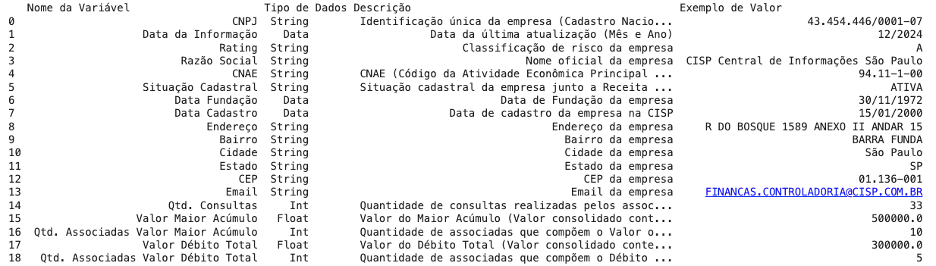
\includegraphics[width=\textwidth]{dicionariodedados.png}
    \caption{Dicionário de Dados Original}
    \label{fig:dicionario_dados}
\end{figure}


A Figura~\ref{fig:dicionario_dados} apresenta o dicionário de dados empregado no estudo, detalhando as variáveis analisadas, seus respectivos tipos de dados, uma breve descrição e exemplos de valores. Esse dicionário desempenhou um papel crucial na estruturação do modelo proposto, contribuindo para a organização e consistência na análise dos dados.

\subsection{Preparação dos Dados}

O primeiro passo na preparação dos dados foi a renomeação de todas as variáveis para o idioma inglês, com o objetivo de facilitar a replicação do estudo por outros pesquisadores e profissionais, ampliando sua acessibilidade e compreensão.

Na sequência, foram aplicadas às variáveis textuais as funções \texttt{str.strip()} e \texttt{str.lower()} em Python, para remover espaços em excesso e padronizar o formato em letras minúsculas. Essas transformações garantiram maior consistência nas informações, reduzindo erros decorrentes de formatos inconsistentes.

Para variáveis relacionadas a datas, foi utilizado \texttt{pd.to\_datetime} (biblioteca Pandas), que converteu os valores em um formato padronizado. O parâmetro \texttt{errors='coerce'} tratou valores inválidos, substituindo-os por nulos (NaT). Além disso, o método \texttt{.dt.normalize()} ajustou as datas ao horário padrão, eliminando informações desnecessárias sobre tempo. Essas mudanças asseguraram uniformidade e integridade dos dados temporais.

No tratamento de variáveis numéricas com valores ausentes, foi utilizado o comando:
\begin{itemize}
    \item \texttt{fillna(0.0).astype(int)}: Substituiu valores nulos por 0.0 e converteu as colunas para o tipo inteiro, garantindo consistência no formato.
\end{itemize}

Variáveis com alta concentração de valores nulos, como \texttt{name}, \texttt{cnae}, \texttt{status}, \texttt{address}, \texttt{city} e \texttt{neighborhood}, apresentaram 59 registros ausentes devido a limitações na fonte de dados (Receita Federal do Brasil). Como esses registros se referiam a CNPJs baixados sem informações adicionais, optou-se por excluí-los, preservando a integridade do \textit{dataset}.

\subsubsection{Criação de Novas Variáveis}

Para validar a hipótese de alterações cadastrais, foram criadas variáveis booleanas: \texttt{addressChanged}, \texttt{nameChanged}, \texttt{emailChanged} e \texttt{cnaeChanged}, indicando alterações nas respectivas informações ao longo do tempo. O processo envolveu:
\begin{enumerate}
    \item Comparação de valores (atual e anterior) para cada cliente;
    \item Identificação de alterações específicas dentro do mesmo \textit{customerID};
    \item Armazenamento dos resultados em colunas booleanas correspondentes.
\end{enumerate}

Além disso, a variável \texttt{customerID} foi anonimizada com o algoritmo \textbf{SHA-256}, e a coluna original foi excluída. A nova coluna \texttt{customer} foi posicionada como a primeira no \textit{dataset}.

\subsubsection{Transformações Relacionadas ao Tempo de Fundação}

Foi criada a variável \texttt{riskFoundation}, classificando empresas com base no número de anos desde sua fundação:
\begin{itemize}
    \item \textbf{High Risk:} Menos de 3 anos;
    \item \textbf{Low Risk:} Mais de 20 anos;
    \item Faixas intermediárias (\textit{Moderate-High, Moderate e Low-Moderate}) refletem níveis progressivos de estabilidade.
\end{itemize}

Para investigar inconsistências entre tempo de atividade e data de fundação, foi criada a variável \texttt{registrationAlert}, que sinaliza casos em que a data de registro diverge do período de atividade esperado.

\subsubsection{Análises de Crescimento Atípico}

Foram desenvolvidas variáveis auxiliares para identificar padrões atípicos:
\begin{enumerate}
    \item \textbf{Comportamento no Volume de Consultas:} A variável \texttt{queriesIncreaseAlert} foi criada ao calcular a média móvel de 3 meses para a variável \texttt{queries} e identificar aumentos superiores a 30\%.
    \item \textbf{Crescimento no Maior Acúmulo:} A variável \texttt{quantityGreaterAccumulationAlert} sinalizou aumentos significativos na variável \texttt{quantityGreaterAccumulation}, com base em uma média móvel de 3 meses e aumento superior a 30\%.
    \item \textbf{Crescimento no Débito Total:} A variável \texttt{quantityDebitAlert} identificou crescimentos atípicos no débito total, seguindo a mesma metodologia.
\end{enumerate}

Após essas análises, colunas auxiliares foram removidas, mantendo o \textit{dataset} enxuto e organizado.

\subsubsection{Normalização e Preparo Final}

Variáveis como \texttt{amountDebit} e \texttt{amountGreaterAccumulation} foram normalizadas com \texttt{np.log1p} para reduzir assimetrias e ajustadas em faixas categóricas (\textit{Very Low, Low, Medium, High}). A análise inicial mostrou distribuições equilibradas após a remoção de \textit{outliers} com base no \textit{Intervalo Interquartil} (IQR).

A variável \texttt{default} foi criada a partir da classificação \texttt{rating}, indicando alto risco de inadimplência (\texttt{True}) para clientes com \texttt{rating} `d' ou `e'. Variáveis como \texttt{customer} e \texttt{updatedMonth} foram removidas por não contribuírem diretamente para a detecção de fraudes financeiras.

\subsubsection{Resultado Final}

Após a preparação, o \textit{dataset} final foi composto pelas seguintes variáveis relevantes, otimizadas para aplicação no modelo \textit{Isolation Forest}, garantindo eficiência na detecção de fraudes financeiras.


Essas etapas resultaram em um \textit{dataset} robusto, focado em variáveis relevantes para a aplicação do modelo \textit{Isolation Forest}, garantindo maior eficiência na detecção de fraudes financeiras.


\subsection{Modelagem}

O estudo utilizou o algoritmo \textit{Isolation Forest}, da biblioteca \textit{Scikit-learn}, para detectar golpes financeiros em operações de crédito realizadas por indústrias de bens de consumo. Esse modelo foi escolhido devido à sua eficiência na identificação de anomalias em grandes volumes de dados, utilizando o conceito de isolamento, onde instâncias anômalas são mais facilmente identificadas em razão de seu comportamento atípico em relação à maioria dos dados.

A implementação do modelo foi precedida por uma preparação rigorosa dos dados, com etapas de normalização, categorização e remoção de \textit{outliers}, garantindo a consistência e a qualidade necessárias para o treinamento. Para transformar variáveis categóricas e booleanas em um formato numérico adequado, foi aplicado o \textit{One-Hot Encoding} utilizando a função \texttt{pd.get\_dummies} da biblioteca Pandas. Esse processo converteu variáveis categóricas em múltiplas colunas binárias, permitindo que o modelo processasse as informações sem introduzir hierarquias artificiais. As variáveis transformadas incluíram aspectos como estado do cliente, alterações cadastrais, alertas e classificações de risco, destacando a variável \texttt{riskFoundation}, que foi codificada em colunas independentes como \texttt{riskFoundation\_High}, \texttt{riskFoundation\_Moderate} e \texttt{riskFoundation\_Low}.

O \textit{Isolation Forest} foi configurado com uma taxa de contaminação de 5\%, que define a proporção esperada de anomalias, e o parâmetro \texttt{random\_state=42} para garantir a reprodutibilidade dos resultados. O modelo foi treinado com o método \texttt{fit}, ajustando-se aos padrões dos dados para identificar instâncias normais e anômalas. Após o treinamento, o método \texttt{predict} classificou cada instância do \textit{dataset}, gerando previsões armazenadas na nova coluna \texttt{anomaly}, onde 1 indica instâncias normais e -1 aponta anomalias.

A análise da coluna \texttt{anomaly} revelou a proporção de instâncias normais e anômalas, permitindo uma visão inicial da distribuição de anomalias no \textit{dataset}. Essa abordagem demonstrou-se eficiente para identificar comportamentos atípicos, contribuindo para a detecção de fraudes financeiras em operações de crédito. A integração de um processo robusto de preparação dos dados com o treinamento do modelo destacou o \textit{Isolation Forest} como uma ferramenta escalável e eficaz para mitigação de riscos financeiros.

\subsection{Avaliação}

Para realizar a avaliação do modelo, o \textit{Isolation Forest} gera predições que classificam as observações como normais (1) ou anomalias (-1). A comparação dessas predições com os rótulos verdadeiros (\texttt{true\_labels}) permite calcular métricas de desempenho, como precisão, \textit{recall}, acurácia e F1-Score. Contudo, como o \textit{dataset} original não possuía rótulos verdadeiros, optou-se por simular rótulos com base em regras de negócio e conhecimento do domínio, considerando a natureza e o contexto dos dados analisados.

Existem várias técnicas para lidar com a ausência de rótulos, como a injeção de anomalias sintéticas ou a avaliação qualitativa das observações classificadas pelo modelo. Neste estudo, a simulação baseada em regras foi escolhida devido à familiaridade com o contexto do \textit{dataset} e à identificação de padrões consistentes em golpes financeiros observados na CISP.

Com base em regras de negócio, foi criada a variável \texttt{true\_labels} no \textit{dataset}, fundamentada em características recorrentes identificadas em casos reais de fraudes financeiras. As principais características observadas foram:

\begin{enumerate}
    \item \textbf{Crescimento Atípico no Volume de Compras:} Representado pelas variáveis \texttt{quantityGreaterAccumulationAlert} e \texttt{quantityDebitAlert}, que assumem o valor \texttt{True} em situações de comportamento anômalo, como um aumento significativo e incomum no volume de compras.

    \item \textbf{Aumento no Comportamento de Consultas:} A variável \texttt{queriesIncreaseAlert}, que sinaliza \texttt{True} quando há um aumento expressivo no número de consultas realizadas, comportamento frequentemente associado a tentativas de golpe.

    \item \textbf{Inconsistência no Tempo de Atividade vs. Data de Fundação:} Alguns CNPJs permaneceram inativos por longos períodos e foram posteriormente reativados sem histórico de relacionamento com indústrias, um comportamento típico em golpes financeiros. Essa característica é representada pela variável \texttt{riskFoundation}, com o valor \texttt{high}.
\end{enumerate}

Essas regras foram aplicadas como critérios para identificar anomalias no \textit{dataset}, resultando na criação de uma base de rótulos (\texttt{true\_labels}) consistente e alinhada ao conhecimento de domínio para a detecção de fraudes financeiras.

Com a aplicação da técnica, o modelo \textit{Isolation Forest} identificou 1.338 casos de anomalias no \textit{dataset}, indicando observações com padrões atípicos e potencialmente fraudulentos.

\subsection{Implantação}

O modelo foi implementado através da criação de um serviço (API), que recebe os dados das solicitações e retorna uma classificação em tempo real. Esse modelo foi integrado ao sistema de motor de crédito atualmente disponibilizado pela CISP aos seus associados. Vale destacar que o fluxo de concessão de crédito descrito já está em operação com os associados, e a inclusão da consulta à API de detecção de golpes financeiros foi a principal novidade incorporada ao processo.

A Figura~\ref{fig:fluxo_credito} ilustra o fluxo de concessão de crédito para os associados da CISP que utilizam o motor de crédito. Esse fluxo operacional segue as etapas descritas a seguir:

\begin{figure}[H]
    \centering
    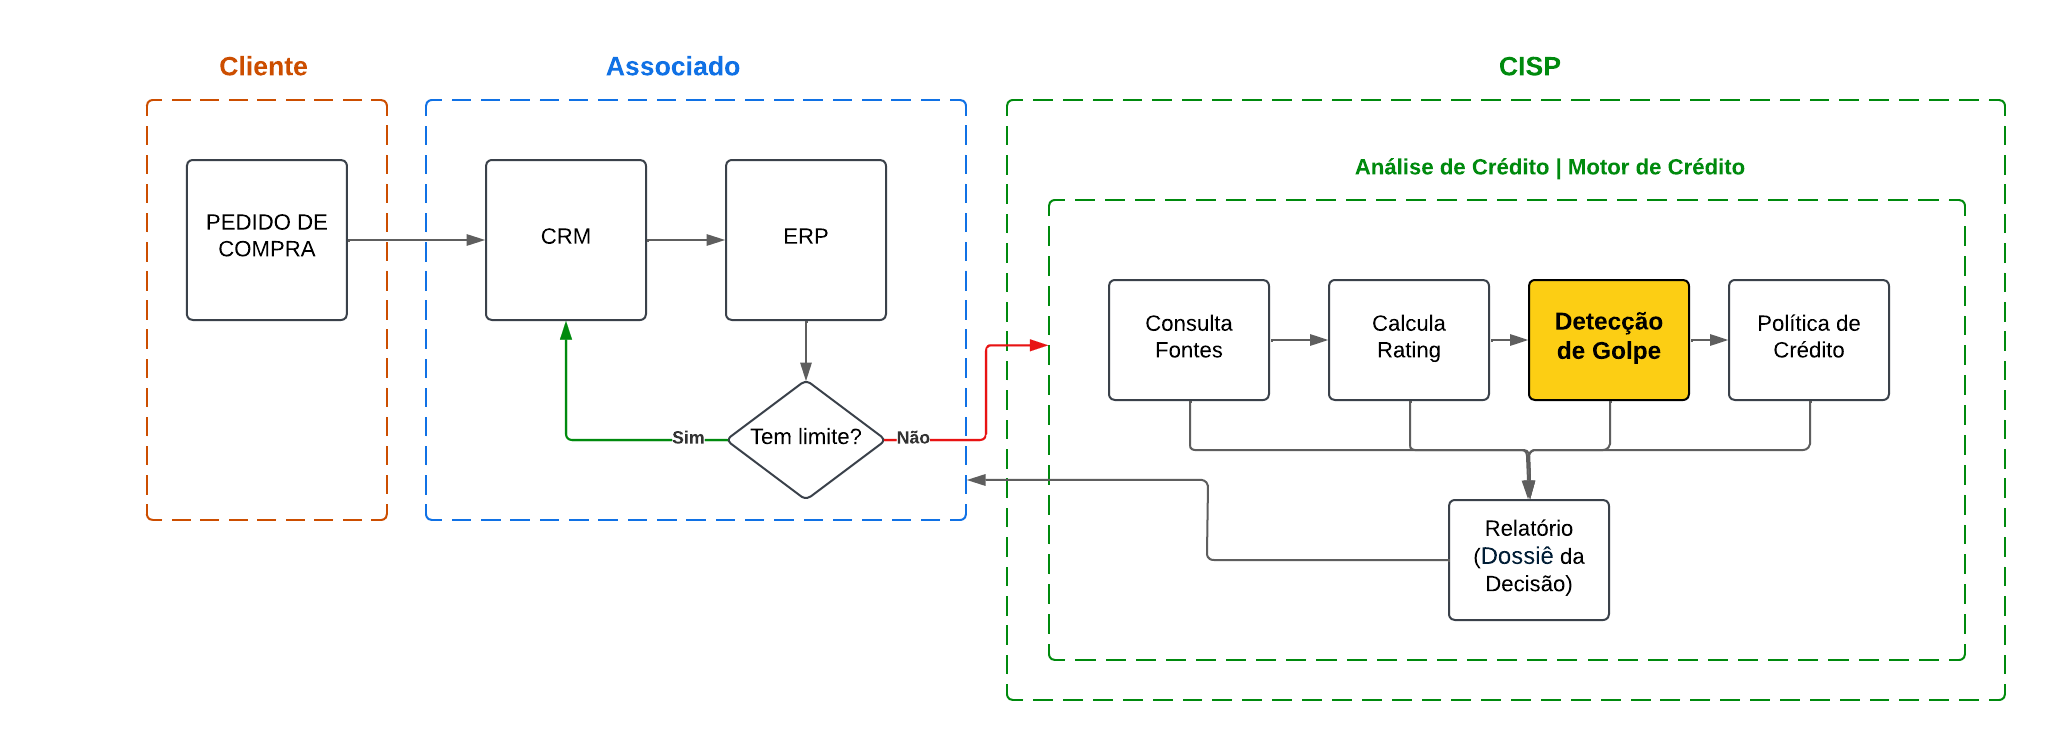
\includegraphics[width=0.8\textwidth]{motordecredito.png}
    \caption{Fluxo de Concessão de Crédito Integrado com a API de Detecção de Golpes}
    \label{fig:fluxo_credito}
\end{figure}


\begin{enumerate}
    \item \textbf{Identificação do Cliente:} 
    Inicialmente, o cliente do associado é identificado como sendo um novo cliente (sem histórico de movimentações com o associado) ou um cliente ativo (com histórico de transações anteriores). O cliente, então, realiza uma solicitação de compra junto ao associado.

    \item \textbf{Consulta Inicial ao ERP:}
    O sistema CRM do associado envia a solicitação ao ERP para verificar se o cliente possui crédito disponível.
    \begin{itemize}
        \item \textbf{Caso tenha crédito suficiente e em vigência:} O pedido de compra é aprovado automaticamente, e o cliente é comunicado.
        \item \textbf{Caso não tenha crédito:} Se o crédito estiver expirado, comprometido ou insuficiente, o ERP encaminha a solicitação ao motor de crédito da CISP para realização de uma análise detalhada.
    \end{itemize}

    \item \textbf{Análise pelo Motor de Crédito da CISP:}
    O motor de crédito da CISP contém todas as regras personalizadas para executar a análise de crédito, de acordo com a política de crédito da empresa associada. O fluxo de análise segue as etapas abaixo:
    \begin{itemize}
        \item \textbf{Consulta às Fontes de Informação:}
        O motor consulta diversas bases de dados, incluindo:
        \begin{itemize}
            \item Dados cadastrais em fontes públicas;
            \item Outras informações definidas previamente pela empresa.
        \end{itemize}
        Como parte das boas práticas de gestão de risco de crédito, as configurações dessas fontes e políticas devem ser alinhadas às diretrizes da política de crédito da empresa.

        \item \textbf{Cálculo do Risco de Performance:} 
        Após a coleta das informações, o motor realiza o cálculo do risco de performance do cliente. Esse cálculo considera aspectos como histórico de crédito e a capacidade de pagamento do cliente.

        \item \textbf{Inclusão da Consulta à API de Detecção de Golpes:} 
        Como novidade no processo, o motor de crédito agora consulta a API de detecção de golpes financeiros, que retorna um resultado indicando se a transação é caracterizada como um possível golpe financeiro ou não.
    \end{itemize}

    \item \textbf{Tomada de Decisão:} 
    Após a conclusão da análise de risco e a verificação contra golpes financeiros, o motor de crédito aplica as regras de tomada de decisão, conforme configurado na política de crédito da empresa associada.
    \begin{itemize}
        \item \textit{Exemplo:} Se o cliente possui uma classificação de rating "boa" e uma alta probabilidade de golpe financeiro, o sistema analisa os critérios de recusa contidos na política de crédito do associado e toma uma decisão automatizada.
    \end{itemize}

    \item \textbf{Geração do Dossiê:} 
    Toda decisão é acompanhada por um dossiê, que reúne diversas informações e relatórios para garantir transparência e rastreabilidade do processo. Esse dossiê inclui dados coletados, resultados das análises e as justificativas para a decisão final.
\end{enumerate}

O fluxo de concessão de crédito já existente nos associados da CISP foi aprimorado com a inclusão da API de detecção de golpes financeiros, adicionando uma camada adicional de proteção contra fraudes. Essa integração não apenas reforçou a gestão de riscos, mas também contribuiu para maior agilidade e precisão nas decisões de crédito automatizadas.

% REFERÊNCIAS
\newpage
\bibliographystyle{abnt-alf}
\bibliography{biblproj} % Certifique-se de que o arquivo biblproj.bib está correto






\end{document}
